\begin{pastexam}[label={px:ncku-114-prog-12}]{成大資訊聯招 114 學年度 第 12 題}
（問答）

{[5\%]} Considering the following B-tree of order 4.

\begin{center}%
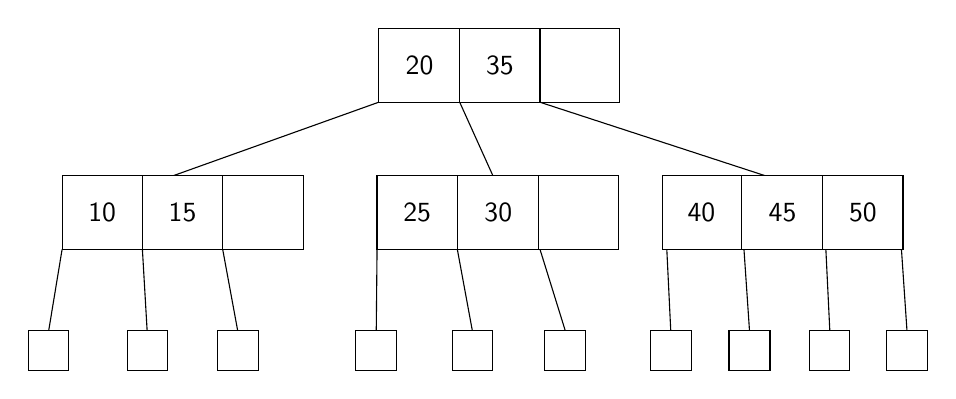
\begin{tikzpicture}[every node/.style={font=\sffamily}]
\draw (4.21,0.00) rectangle (7.27,-0.94);
\draw (5.24,0.00) -- (5.24,-0.94);
\draw (6.26,0.00) -- (6.26,-0.94);
\node at (4.73,-0.47) {20};
\node at (5.75,-0.47) {35};
\draw (0.19,-1.87) rectangle (3.26,-2.81);
\draw (1.21,-1.87) -- (1.21,-2.81);
\draw (2.23,-1.87) -- (2.23,-2.81);
\node at (0.70,-2.34) {10};
\node at (1.72,-2.34) {15};
\draw (4.19,-1.87) rectangle (7.26,-2.81);
\draw (5.21,-1.87) -- (5.21,-2.81);
\draw (6.24,-1.87) -- (6.24,-2.81);
\node at (4.70,-2.34) {25};
\node at (5.73,-2.34) {30};
\draw (7.81,-1.87) rectangle (10.87,-2.81);
\draw (8.82,-1.87) -- (8.82,-2.81);
\draw (9.85,-1.87) -- (9.85,-2.81);
\node at (8.31,-2.34) {40};
\node at (9.34,-2.34) {45};
\node at (10.36,-2.34) {50};
\draw (4.21,-0.94) -- (1.61,-1.87);
\draw (5.24,-0.94) -- (5.66,-1.87);
\draw (6.26,-0.94) -- (9.11,-1.87);
\draw (0.19,-2.81) -- (0.02,-3.84);
\draw (-0.24,-3.84) rectangle (0.27,-4.35);
\draw (1.21,-2.81) -- (1.27,-3.84);
\draw (1.02,-3.84) rectangle (1.53,-4.35);
\draw (2.23,-2.81) -- (2.42,-3.84);
\draw (2.16,-3.84) rectangle (2.68,-4.35);
\draw (4.19,-2.81) -- (4.18,-3.84);
\draw (3.92,-3.84) rectangle (4.44,-4.35);
\draw (5.21,-2.81) -- (5.40,-3.84);
\draw (5.15,-3.84) rectangle (5.66,-4.35);
\draw (6.26,-2.81) -- (6.58,-3.84);
\draw (6.32,-3.84) rectangle (6.84,-4.35);
\draw (7.87,-2.81) -- (7.92,-3.84);
\draw (7.66,-3.84) rectangle (8.18,-4.35);
\draw (8.85,-2.81) -- (8.92,-3.84);
\draw (8.66,-3.84) rectangle (9.18,-4.35);
\draw (9.89,-2.81) -- (9.94,-3.84);
\draw (9.68,-3.84) rectangle (10.19,-4.35);
\draw (10.85,-2.81) -- (10.92,-3.84);
\draw (10.66,-3.84) rectangle (11.18,-4.35);
\end{tikzpicture}%
\end{center}
\smallskip

Successively insert 62, 5, 85, and 12 one at a time into the above B-tree and then delete 5, 50, 62, 85, and 10 one at a time. Please show the new tree after completing all the insertion and deletion operations.
\end{pastexam}

\begin{pastsoln}
答案：最後的 B 樹只有兩層：根 $[20, 35]$，三個葉子 $[12, 15]$、$[25, 30]$、$[40, 45]$（圖見最後）。

\textbf{規則}（資結書第~11.2~節）。 $4$ 階 B 樹每個節點最多 $3$ 個鍵、$4$ 個子節點；非根節點至少 $\lceil 4/2 \rceil - 1 = 1$ 個鍵。
插入：放進葉子，到 $4$ 個鍵 $k_1 < k_2 < k_3 < k_4$ 時分裂，$k_{\lceil 4/2 \rceil} = k_2$ 往上送，$k_1$ 留下，$k_3, k_4$ 成為新節點。
刪除：內部節點的鍵用後繼取代；節點不足時先向右兄弟借、再向左兄弟借，都不能借就合併（有右兄弟就和右兄弟合併）。 下面用
$[\ldots]\{\ldots\}$ 表示一個節點和它的子節點。

\textbf{插入}：
\begin{enumerate}
\item \textbf{$62$}：放進 $[40, 45, 50]$ 成為 $[40, 45, 50, 62]$，溢位。 $45$ 上升，分成 $[40]$、$[50, 62]$。 根變成 $[20, 35, 45]$，
子節點 $[10, 15]$、$[25, 30]$、$[40]$、$[50, 62]$。
\item \textbf{$5$}：$[10, 15] \to [5, 10, 15]$。
\item \textbf{$85$}：$[50, 62] \to [50, 62, 85]$。
\item \textbf{$12$}：$[5, 10, 15] \to [5, 10, 12, 15]$，溢位，$10$ 上升，分成 $[5]$、$[12, 15]$。 根變成 $[10, 20,$ $35, 45]$，也溢位：$20$
上升成為新的根，分成 $[10]\{[5], \allowbreak [12, 15]\}$ 和 $[35, 45]\{[25, 30], \allowbreak [40], \allowbreak [50, 62, 85]\}$。 樹高變成 $3$ 層。
\end{enumerate}

\textbf{刪除}：
\begin{enumerate}
\item \textbf{$5$}：葉子 $[5]$ 變空。 右兄弟 $[12, 15]$ 有 $2$ 個鍵，可以借：分隔鍵 $10$ 下來，$12$ 上去。 左半邊變成
$[12]\{[10], \allowbreak [15]\}$。
\item \textbf{$50$}：$[50, 62, 85] \to [62, 85]$。
\item \textbf{$62$}：$[62, 85] \to [85]$。
\item \textbf{$85$}：$[85]$ 變空。 它是 $[35, 45]$ 的最後一個子節點，沒有右兄弟；左兄弟 $[40]$ 只有 $1$ 個鍵，不能借，和左兄弟合併：
$40$、分隔鍵 $45$ 合成 $[40, 45]$。 父節點變成 $[35]\{[25, 30], \allowbreak [40, 45]\}$，還有 $1$ 個鍵，夠。
\item \textbf{$10$}：$[10]$ 變空。 右兄弟 $[15]$ 只有 $1$ 個鍵，不能借；沒有左兄弟。 和右兄弟合併：$[12, 15]$，父節點 $[12]$ 少了
一個鍵而變空。 這個空節點的右兄弟 $[35]$ 只有 $1$ 個鍵，不能借，再合併：空節點、根的分隔鍵 $20$、$[35]$ 合成 $[20, 35]$，子節點
$[12, 15]$、$[25, 30]$、$[40, 45]$。 根因此變空，拿掉，$[20, 35]$ 成為新的根，樹高回到 $2$ 層。
\end{enumerate}

\begin{center}
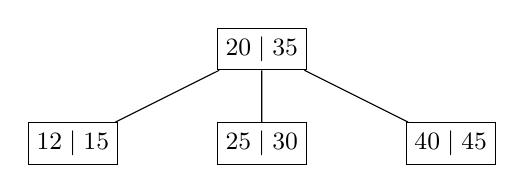
\begin{tikzpicture}[k/.style={draw,rectangle,inner sep=3pt,minimum height=5mm,font=\small}]
\node[k] (r) at (3,0) {$20 \mid 35$};
\node[k] (a) at (0.6,-1.2) {$12 \mid 15$};
\node[k] (b) at (3,-1.2) {$25 \mid 30$};
\node[k] (c) at (5.4,-1.2) {$40 \mid 45$};
\draw (r)--(a) (r)--(b) (r)--(c);
\end{tikzpicture}
\end{center}
這一題換成另一種常見的約定（分裂時上升 $k_3$，或刪除時先向左兄弟借），中間過程會不一樣，但最後的樹相同：用 $k_3$ 上升時，
插入 $62$ 會得到 $[20, 35, 50]\{\ldots, [40, 45], \allowbreak [62]\}$，一路做完最後仍是根 $[20, 35]$、葉子 $[12, 15]$、$[25, 30]$、$[40, 45]$。
\end{pastsoln}
